\documentclass[10pt,twocolumn]{article}

\usepackage[margin=0.85in]{geometry}
\usepackage{amsmath,amssymb}
\usepackage{booktabs}
\usepackage{microtype}
\usepackage{xcolor}
\usepackage{tikz}
\usepackage{pgfplots}
\pgfplotsset{compat=1.16}
\usetikzlibrary{arrows.meta,positioning,shapes.geometric,backgrounds,fit,calc}
\usepackage[hidelinks]{hyperref}
\usepackage{pifont}
\usepackage{caption}
\captionsetup{font=small,labelfont=bf}

% palette (shared with the pillar-UDP / message-format papers)
\definecolor{pgood}{RGB}{31,119,80}
\definecolor{pbad}{RGB}{200,40,40}
\definecolor{pnode}{RGB}{38,70,120}
\definecolor{pcell}{RGB}{235,240,248}
\definecolor{pcellb}{RGB}{240,247,240}
\definecolor{pgray}{RGB}{110,110,110}
\definecolor{pmid}{RGB}{210,140,20}

\newcommand{\code}[1]{\texttt{\small #1}}
\newcommand{\Cid}{\code{Cid}}
\newcommand{\hlc}[1]{\ensuremath{t_{#1}}}

\tikzset{
  box/.style={rectangle,rounded corners=2pt,draw=pnode,thick,fill=white,
              align=center,font=\footnotesize,inner sep=4pt},
  seal/.style={box,fill=pcell},
  flow/.style={-{Stealth[length=2mm]},thick,pnode},
}

\title{\vspace{-3.5em}\bfseries The Pillar Data Layer: A Multi-Model Streaming
Database Turned Inside-Out for a Trustless Federation}
\author{\normalsize pillar engineering \quad(machine-checked design note)}
\date{\normalsize 2026-09-14}

\begin{document}
\maketitle

\begin{abstract}
\noindent
Samza and Kleppmann's ``turning the database inside out'' showed that an immutable
log of events plus materialized views folded from it is a better factoring than a
mutable-state database: the log is the source of truth, views are derived, and caches
and indexes stop being things you invalidate by hand and become things you
\emph{rebuild}. Samza did this inside a trusted datacenter on a central broker
(Kafka). Pillar does the same factoring for a \textbf{trustless, serverless,
cryptographically-verifiable federation of PGP-trusted peers}---no broker, every
record signed and content-addressed, confidentiality and authorization in the record
format, convergence and coordination model-checked in TLA\textsuperscript{+}. The
user-visible consequence, and the point of this note, is that Pillar offers users the
\emph{same} data primitives it builds itself out of, over the \emph{same} substrate
(the \code{PillarMessage} envelope), with a real inspect/query surface---there is no
separate ``user database'' bolted next to bespoke internal stores. We specify a small,
distinct primitive suite (a \textbf{keyed store} with K/V and Document surfaces,
\textbf{SQL views} as a derived-read layer over it, and a \textbf{time-series}
store), show how SQL over the document store works as catalog-as-data with
append-only field-delta writes and migration-free schema change, place the one hard
consistency requirement (a CP subset) as a Samza co-partition-and-fold ordered by the
coordination core rather than a global lock, and fix the data-placement boundary at
the \emph{collection} so every layer inherits one pinning decision over node tags. A
time-sequence diagram walks the common and the distinctive streamdb operations---write
and gossip merge, concurrent last-writer-wins convergence, a CP exclusive admission,
a query from a folded view, a new view over existing data, and content-addressed
rehydrate. This note is the design of record; the original-design core is
TLA\textsuperscript{+}-gated per Pillar's specify-then-build rule.
\end{abstract}

\section{The inside-out thesis, for a trustless federation}
The inside-out model inverts the database: instead of a mutable table mutated in
place, an append-only log of immutable events is the source of truth, and every
readable view is a deterministic fold of that log. Samza realized this on Kafka
inside a trusted datacenter. Pillar keeps the factoring but changes the environment
to a peer-to-peer federation with no central owner and no trusted operator, and adds
what that environment demands: every op is content-addressed (a real CIDv1
multihash) and signed by a PGP-rooted identity; reads and writes gate through a
Web-of-Trust RBAC decider; bodies are cell-encrypted or recipient-sealed; and the
convergence, ordering, coordination, and confidentiality invariants are model-checked
in TLA\textsuperscript{+} before any Rust. The doctrine that organizes the rest of
this note: \textbf{build each data primitive once, dogfood it internally, and offer
it to users with a real inspect/query surface}---so each internal plane (manifests,
RBAC, sessions, quota, identity, observability) is a \emph{consumer} of the same
primitives a user application consumes.

\section{One substrate, one envelope}
Everything in the data layer rides one substrate. The event log is a
content-addressed CvRDT op-log (\code{pillar-streamdb}): each op is immutable,
content-addressed, signed, and merged by set-union; a deterministic fold produces the
materialized view. There is exactly one record on the wire and on disk---the
\code{PillarMessage} envelope (\code{pillar-wire}, companion paper)---of which streamdb
ops, observability signals, and every libp2p control message are variants; the
convergent cell-seal keeps the \Cid{} stable under encryption. The \emph{hot path} is
pubsub/gossip of these envelopes; the \emph{cold/bootstrap path} is Pillar's own
embedded IPFS node (\code{pillar-ipfs}), content-addressed and self-hosted, off the
public DHT. A restarting or new node rehydrates from IPFS-pinned sealed segments plus
its custody-held key---there is no central broker to replay from. Everything below is
a \emph{model over this one substrate}: the ``different databases'' a user sees are
different fold/query/retention disciplines over the same signed log, not different
storage systems.

\section{The primitive suite}
An application does not need one storage primitive per CRDT type, nor nine different
stores; it needs a small number of distinct \emph{access patterns}. Pillar offers
three query interfaces over two storage models over the one substrate
(Table~\ref{tab:suite}).

\begin{table}[t]
\centering\small
\begin{tabular}{@{}p{0.30\linewidth}p{0.62\linewidth}@{}}
\toprule
\textbf{Storage model} & \textbf{Access pattern / discipline}\\
\midrule
Keyed store\newline(K/V + Document surfaces) & point lookup / structured record;
per-field LWW-register by HLC; AP default, CP opt-in; snapshot + log-tail replay,
folds to a condensable current state\\
Time-series (TSDB) & time-windowed range, retention/downsample, past-query required;
append-only immutable blocks, \emph{no} condensable current state\\
\midrule
\textbf{Query interface} & \textbf{Over}\\
\midrule
Keyed get/scan/watch & the keyed store (point + prefix + subscribe)\\
SQL views & the keyed store, as a \emph{derived-read} layer owning no storage:
project/filter/join/aggregate/traverse into cached materialized views\\
PSL & the TSDB (the compact-text/structured signal query surface)\\
\bottomrule
\end{tabular}
\caption{The suite a user picks: two storage models, three query interfaces, one
substrate. Both storage models persist to the \emph{same} IPFS content store---what
differs is the data model on top.}
\label{tab:suite}
\end{table}

\textbf{SQL is a query layer, not a third stored type.} It holds no storage; it folds
the keyed store's collections into materialized views and caches them. Counters
(\code{SUM}/\code{GROUP BY}), graph traversals (recursive joins over an edge
collection), and rollups are \emph{queries}, not primitives. There is no graph
database, no standalone counter, and no ``log store'' distinct from the substrate---the
streamdb \emph{is} the log. \textbf{Cache is not a user primitive} either: it is the
$(\text{query},\text{root})$-keyed materialized-view cache that recomputes only when
the source root changes, invisible in the user's model.

\section{SQL over the document store}
The relational surface presents mutable flat rows, but storage is the append-only
signed log; the illusion is maintained by folding.

\paragraph{The catalog is data.} DDL is not special---it writes documents to a
\code{\_\_catalog} system collection, event-sourced and gossip-replicated like
everything else. \code{CREATE TABLE app.users(\dots)} writes a table document
\code{\{schema,collection:'app.users'\}}; \code{CREATE MATERIALIZED VIEW} writes a
view document \code{\{source:['app.users'],query,since\}}. A node learns every
database/table/view by folding \code{\_\_catalog}.

\paragraph{Data\,$\to$\,table is structural.} A row's key \emph{is}
\code{(collection,id)}: the collection component is the table id, so a node never
needs a side lookup to know which table a document belongs to. The op-log is indexed
by collection (and indexed columns) so folding a table is not a full scan.

\paragraph{A row update appends a delta, never mutating a flat document.} An
\code{UPDATE} compiles to a \code{put} op carrying \emph{only} the changed fields with
an HLC. The flat row is derived by folding the key's ops under per-field LWW:
\begin{quote}\footnotesize
\code{op1 \hlc1: put users/alice \{name:Alice, email:a@x, role:admin\}}\\
\code{op2 \hlc2: put users/alice \{email:alice@y\}}\\
$\Rightarrow$ \code{\{name:Alice(\hlc1), email:alice@y(\hlc2), role:admin(\hlc1)\}}
\end{quote}
Because each field is its own LWW-register, a single-column update rewrites nothing
else, and concurrent updates to \emph{different} fields both survive; same-field
conflicts resolve by highest HLC. \code{DELETE} appends a tombstone; the view drops
the row, the log keeps the event, and compaction later collapses tombstoned keys out
of the snapshot. The only literally-flat stored artifacts---the in-memory view and
the periodic snapshot segment---are derived and rebuildable, never edited in place.

\paragraph{Data\,$\to$\,view is derived, not stored.} A node serving a view does not
consult per-document ``which view?'' pointers. It reads the view document, folds the
source collection(s), applies the predicate/projection, and caches on
$(\text{view-id},\text{root(source)})$. \emph{Views subscribe to sources; sources are
oblivious to views.}

\paragraph{A new view over existing data needs no migration.} A schema change is a new
view over the unchanged source: \code{CREATE MATERIALIZED VIEW app.users\_v2 AS SELECT
id, name AS full\_name, email FROM app.users}. Nothing is moved. Because
\code{app.users}'s ops are immutable and content-addressed, the node building
\code{users\_v2} folds those same ops from the beginning (snapshot + log-tail) under
the new projection; old and new views coexist and consumers cut over gradually.
Missing columns are computed/defaulted in the projection or supplied by a
non-destructive per-field backfill that merges by LWW without rewriting existing
fields.

\section{Ordering: HLC is a wire-format requirement}
\code{OpLog::order} sorts by content-address, not time. That is fine for a grow-only
set, but per-field LWW and any latest-write-wins semantics are arbitrary without a
logical clock in the op payload. Every keyed-store \code{put}/tombstone op therefore
carries a Hybrid Logical Clock timestamp, and the fold resolves same-field conflicts
by highest HLC with a deterministic tiebreak (author/\Cid{}). This is a user-visible
part of the op schema, gated with the wire format.

\section{Consistency: AP by default, a CP subset by co-partitioned fold}
Pillar chooses its CAP point \emph{per view}. The AP majority---sessions, offers,
manifests, config, user records, trust edges---is a CRDT keyed store: writes always
succeed and merge on heal (\code{ViewPolicy::Relaxed}). The handful of genuine hard
invariants---exactly-once admission, hard quota ceilings, uniqueness---are \emph{not}
a relational engine, a global lock, or foreign keys. They are Samza's
co-partition-and-fold: the invariant's key goes in a \code{ViewPolicy::Strict}
partition and the reducer enforces the invariant over that partition's total order.
The one Pillar-specific twist is that Samza gets per-partition total order for free
from Kafka's single leader per partition, whereas Pillar's substrate is
\emph{leaderless}; a Strict partition therefore takes its total order from the
\textbf{coordination core}---a quorum-fenced lease
(\code{CoordinationCore.tla}, \code{AtMostOneHolderPerEpoch})---the direct analog of a
Kafka partition leader, per-key and scoped, never a global lock. A minority partition
starves rather than splitting the brain; safety is absolute, availability is
sacrificed only in the minority and only for the CP subset.

\section{A time sequence of streamdb operations}
Figure~\ref{fig:seq} orders the common and the distinctive streamdb operations in
time across a client, two replica/voter nodes, the streamdb substrate
(pubsub tip + IPFS segments), and a third node that joins with an empty disk.
\ding{182}~A \textbf{write} is a signed, content-addressed \code{put} appended by the
ingress node and gossiped as a tip; a peer merges it by set-union and folds it under
per-field LWW. \ding{183}~A \textbf{concurrent write} to the same field from the peer
carries a higher HLC; with no coordination, set-union merge plus highest-HLC-wins
converges both nodes to the identical row---the CvRDT property that a broker buys with
a single leader, Pillar buys with content-addressing and an HLC. \ding{184}~A
\textbf{CP exclusive} op (a uniqueness \code{INSERT} or a hard quota decrement) is
gated: the ingress acquires a quorum-fenced grant for that key's Strict partition
before the reducer admits it---a per-key lease, not a global lock. \ding{185}~A
\textbf{query} is served from the locally folded materialized view via the
$(\text{query},\text{root})$ cache; any node that pins the sources answers
identically. \ding{186}~A \textbf{new view over existing data} folds the unchanged,
content-addressed source log from snapshot\,+\,tail---no migration, old and new
coexist. \ding{187}~A \textbf{bootstrap} node with an empty disk rehydrates by
fetching the snapshot segment and log tail from \emph{any} peer over IPFS and
unsealing with its custody-held key. Modeled against the streamdb and coordination-core
specifications.

\begin{figure*}[t]
\centering
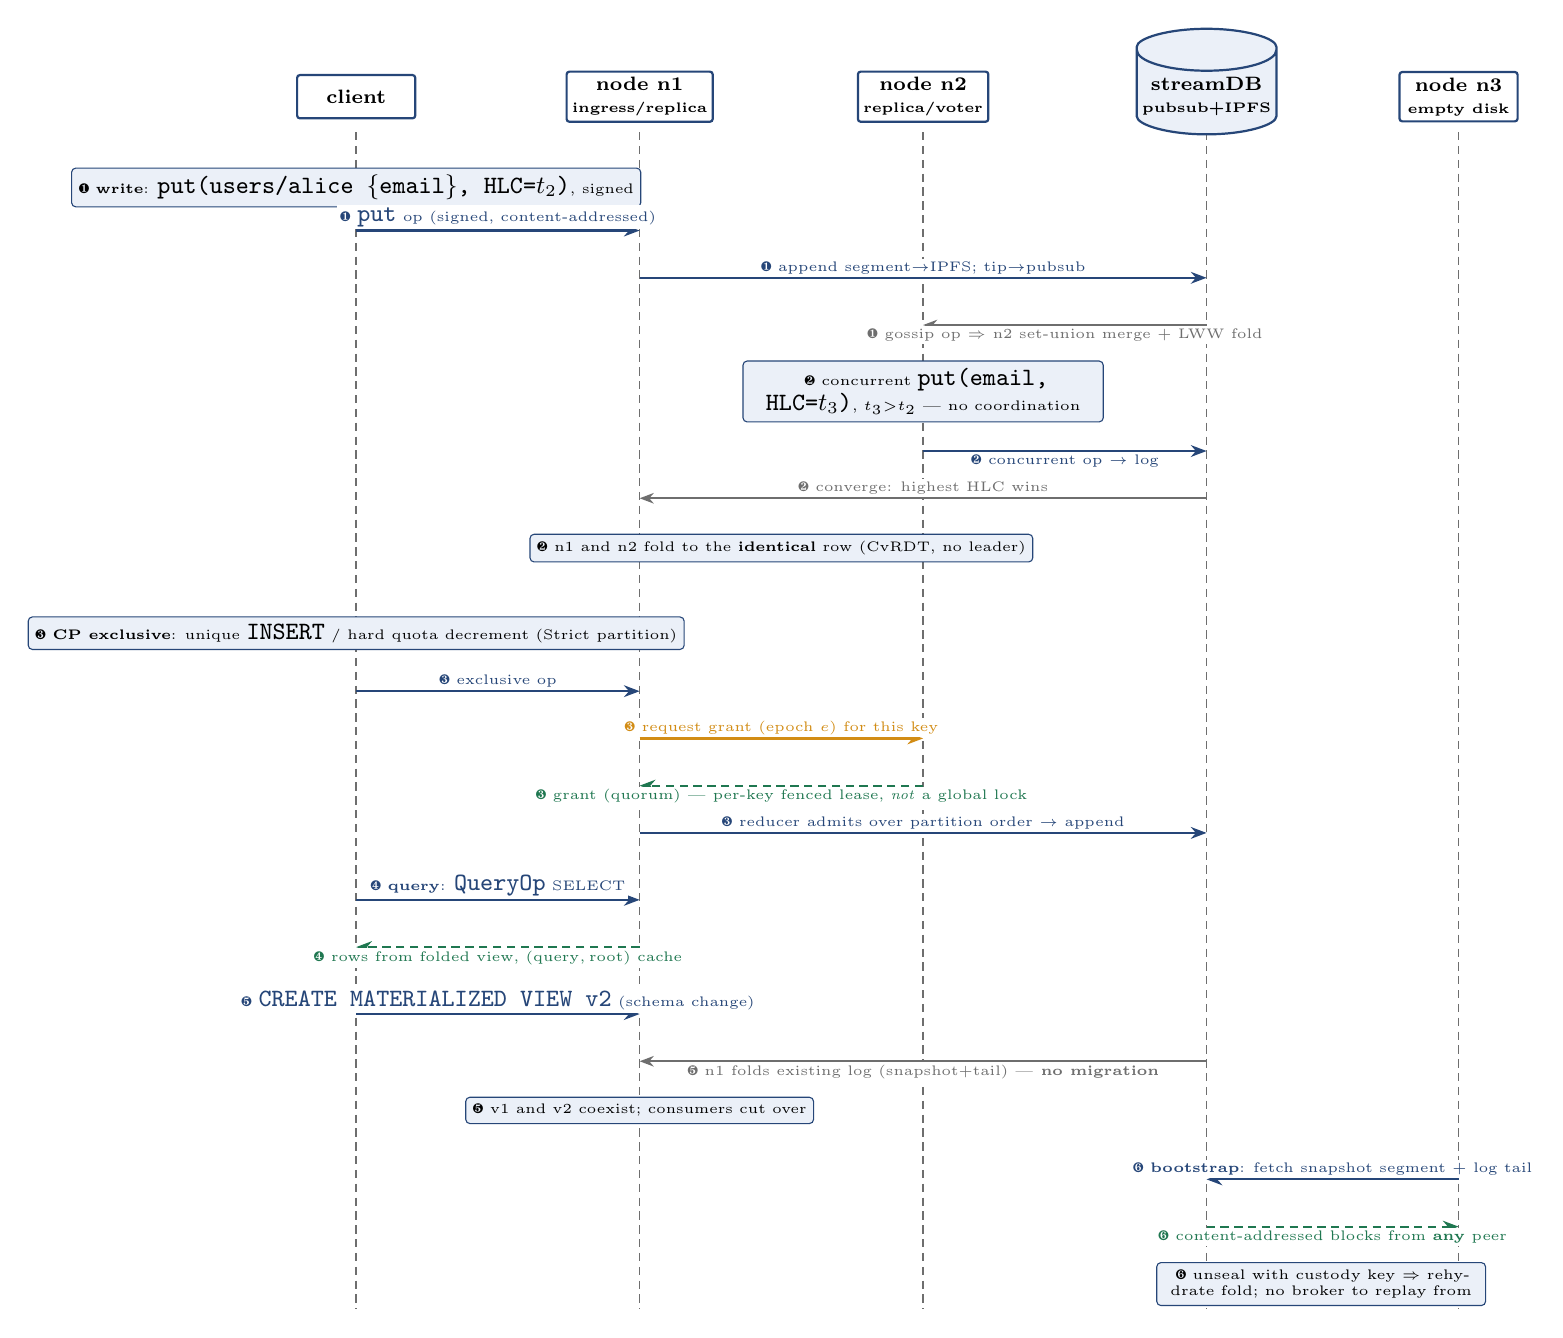
\begin{tikzpicture}[
  part/.style={rectangle,rounded corners=1pt,draw=pnode,thick,fill=white,
               font=\scriptsize\bfseries,minimum height=5.5mm,minimum width=15mm,
               align=center,inner sep=2pt},
  life/.style={pgray,densely dashed,semithick},
  msg/.style={-{Stealth[length=2mm]},thick,pnode},
  ret/.style={-{Stealth[length=2mm]},thick,pgood,densely dashed},
  cp/.style={-{Stealth[length=2mm]},thick,pmid},
  rev/.style={-{Stealth[length=2mm]},thick,pbad},
  cvg/.style={-{Stealth[length=1.8mm]},semithick,pgray},
  lbl/.style={midway,above,font=\tiny,fill=white,inner sep=1pt},
  lblb/.style={midway,below,font=\tiny,fill=white,inner sep=1pt},
  note/.style={rectangle,rounded corners=1.5pt,draw=pnode,fill=pcell,
               font=\tiny,align=center,inner sep=2.5pt}]
  % ---- lifelines (x positions) ----
  \def\xC{0}    \def\xA{3.6}  \def\xB{7.2}  \def\xD{10.8} \def\xE{14.0}
  \def\ybot{-15.4}
  \foreach \x in {\xC,\xA,\xB,\xD,\xE}
     \draw[life] (\x,-0.45) -- (\x,\ybot);
  % ---- participant headers ----
  \node[part] at (\xC,0) {client};
  \node[part] at (\xA,0) {node n1\\{\tiny ingress/replica}};
  \node[part] at (\xB,0) {node n2\\{\tiny replica/voter}};
  \node[part,shape=cylinder,shape border rotate=90,aspect=0.3,fill=pcell] at (\xD,0)
     {streamDB\\{\tiny pubsub+IPFS}};
  \node[part] at (\xE,0) {node n3\\{\tiny empty disk}};
  % ==== 1. WRITE ====
  \node[note,anchor=north] at (\xC,-0.9)
     {\ding{182} \textbf{write}: \code{put(users/alice \{email\}, HLC=\hlc2)}, signed};
  \draw[msg] (\xC,-1.7) -- node[lbl]{\ding{182} \code{put} op (signed, content-addressed)} (\xA,-1.7);
  \draw[msg] (\xA,-2.3) -- node[lbl]{\ding{182} append segment$\to$IPFS; tip$\to$pubsub} (\xD,-2.3);
  \draw[cvg] (\xD,-2.9) -- node[lblb]{\ding{182} gossip op $\Rightarrow$ n2 set-union merge + LWW fold} (\xB,-2.9);
  % ==== 2. CONCURRENT LWW ====
  \node[note,anchor=north,text width=44mm] at (\xB,-3.35)
     {\ding{183} concurrent \code{put(email, HLC=\hlc3)}, \hlc3$>$\hlc2 --- no coordination};
  \draw[msg] (\xB,-4.5) -- node[lblb]{\ding{183} concurrent op $\to$ log} (\xD,-4.5);
  \draw[cvg] (\xD,-5.1) -- node[lbl]{\ding{183} converge: highest HLC wins} (\xA,-5.1);
  \node[note,anchor=north] at ($(\xA,-5.55)!0.5!(\xB,-5.55)$)
     {\ding{183} n1 and n2 fold to the \textbf{identical} row (CvRDT, no leader)};
  % ==== 3. CP EXCLUSIVE ====
  \node[note,anchor=north] at (\xC,-6.6)
     {\ding{184} \textbf{CP exclusive}: unique \code{INSERT} / hard quota decrement (Strict partition)};
  \draw[msg] (\xC,-7.55) -- node[lbl]{\ding{184} exclusive op} (\xA,-7.55);
  \draw[cp] (\xA,-8.15) -- node[lbl]{\ding{184} request grant (epoch $e$) for this key} (\xB,-8.15);
  \draw[ret] (\xB,-8.75) -- node[lblb]{\ding{184} grant (quorum) --- per-key fenced lease, \emph{not} a global lock} (\xA,-8.75);
  \draw[msg] (\xA,-9.35) -- node[lbl]{\ding{184} reducer admits over partition order $\to$ append} (\xD,-9.35);
  % ==== 4. QUERY ====
  \draw[msg] (\xC,-10.2) -- node[lbl]{\ding{185} \textbf{query}: \code{QueryOp} SELECT} (\xA,-10.2);
  \draw[ret] (\xA,-10.8) -- node[lblb]{\ding{185} rows from folded view, $(\text{query},\text{root})$ cache} (\xC,-10.8);
  % ==== 5. NEW VIEW OVER EXISTING DATA ====
  \draw[msg] (\xC,-11.65) -- node[lbl]{\ding{186} \code{CREATE MATERIALIZED VIEW v2} (schema change)} (\xA,-11.65);
  \draw[cvg] (\xD,-12.25) -- node[lblb]{\ding{186} n1 folds existing log (snapshot+tail) --- \textbf{no migration}} (\xA,-12.25);
  \node[note,anchor=north] at (\xA,-12.7)
     {\ding{186} v1 and v2 coexist; consumers cut over};
  % ==== 6. BOOTSTRAP / REHYDRATE ====
  \draw[msg] (\xE,-13.75) -- node[lbl]{\ding{187} \textbf{bootstrap}: fetch snapshot segment + log tail} (\xD,-13.75);
  \draw[ret] (\xD,-14.35) -- node[lblb]{\ding{187} content-addressed blocks from \textbf{any} peer} (\xE,-14.35);
  \node[note,anchor=north east,text width=40mm] at ($(\xE,-14.8)+(0.35,0)$)
     {\ding{187} unseal with custody key $\Rightarrow$ rehydrate fold; no broker to replay from};
\end{tikzpicture}
\caption{\textbf{Time sequence of streamdb operations}, time flowing downward.
\ding{182}~write + gossip merge; \ding{183}~concurrent same-field write converging by
highest-HLC last-writer-wins with no coordination (the distinctive CvRDT property);
\ding{184}~a CP exclusive admission gated on a per-key quorum-fenced lease from the
coordination core, not a global lock; \ding{185}~a query served from a folded,
root-cached materialized view; \ding{186}~a new view built over the unchanged
content-addressed source log with no migration; \ding{187}~a fresh node rehydrating
from IPFS-pinned snapshot + tail fetched from any peer and unsealed with its custody
key. Common operations (\ding{182},\ding{185}) and Pillar-unique ones
(\ding{183},\ding{184},\ding{186},\ding{187}) ride the one \code{PillarMessage}
substrate.}
\label{fig:seq}
\end{figure*}

\section{Placement: the collection is the pinning boundary}
Not every cell node must serve every collection; users isolate data to specific nodes
for performance, security, or other reasons. Every layer---events, K/V, document, SQL,
TSDB---inherits one placement decision because each is a fold of a collection's event
stream, so the \textbf{collection} is the pinning unit: pin a collection on a node and
that node can serve its document view, its TSDB blocks, and any SQL view whose sources
it also holds.

The default (no selector) pins a collection across the \emph{entire cell}: the cell is
the replication set, and there is no separate replication-factor knob (it would raise
meaningless warnings on small clusters and duplicate what cell membership already
expresses). Isolation is opt-in via a \code{CollectionPlacement} resource that selects
nodes by \emph{tag}, reusing the existing attested topology-label machinery that RBAC
targets already use; an empty selector means the whole cell. Views follow their
sources: a materialized view is servable on a node iff that node pins all of the
view's source collections, so placing a view expands to co-pinning its sources---a
node never holds a view without its data. The cell remains the confidentiality
boundary; placement only narrows within a cell. The CLI/UI surfaces, per collection,
its placement tags and the live count and list of participating nodes.

\section{What Pillar has that Samza, Kafka, and Mongo do not}
Honestly, including where Pillar loses. \textbf{Advantages:} no broker and leaderless
(the log is a P2P-gossiped CvRDT, nothing central to run or trust);
cryptographically verifiable and tamper-evident (content-addressed Merkle-DAG,
per-author hash chains and signatures, so a faulty node is detected); identity,
authorization, and encryption in the record format rather than bolted-on ACLs over a
trusted operator; a per-stream CAP knob with model-checked convergence and
heal-after-partition rather than Kafka's CP-only partitions; formal verification in
TLA\textsuperscript{+}; content-addressed durability you self-host (embedded IPFS, off
the public DHT), so a consumer bootstraps from any peer with free dedup and no broker
to replay from; one envelope and one substrate unifying log, state store, query, and
durability instead of five wired-together systems; native subscribe/verify where a
client checks a view's tip itself; and federation/mobility over NAT-traversing libp2p
rather than a datacenter-LAN assumption. \textbf{Where Pillar loses:} throughput and
latency (signing, sealing, content-addressing, and gossiping per op is heavier than a
tuned Kafka append, and Pillar is young and unproven at scale); the conflict model
(per-field LWW is weaker than a single-leader total order for some workloads); and
maturity (formal proofs are not production hours). Net: Pillar wins on
decentralization, verifiability, built-in identity/crypto, formal correctness, and
multi-model unification, and does not win on raw throughput or maturity---Samza's
architecture minus the broker, plus cryptographic trust, plus a unified
state/query/durability layer.

\section{Performance is a standing discipline}
The crypto layer (sign + seal + content-address per op) is real per-op overhead and
the acknowledged price of the guarantees above; the gap to a plaintext broker is
closed by engineering \emph{within} the safety envelope, never by weakening a
guarantee. A recurring (daily) self-perpetuating task measures streamdb op
throughput/latency and view-fold cost against a tracked baseline on a fixed harness
and, on a regression or headroom, files concrete tuning follow-ups---removing
redundant hot-path copies/serializations, fusing envelope construction with signing,
hardware-accelerated hashing and AEAD (AES-NI/AVX), Ed25519 batch verification, a
verify-cache keyed on \Cid{}, zero-copy segment I/O, and batching ops per gossip
round. The hard invariant on every tuning task: no change may weaken a guarantee
(verifiability, per-op signing, content-addressing, or the per-stream CAP posture); a
``speedup'' that drops a signature, a hash check, or a seal is a bug, not an
optimization.

\section{Verification posture}
Consistent with Pillar's specify-then-build rule, the original-design core of this
data layer is TLA\textsuperscript{+}-gated before it is trusted: the streamdb CvRDT and
its fold, the keyed-store op schema including the HLC ordering rule, the coordination
core that orders the CP subset, and the confidentiality/seal invariants of the wire
format. The SQL/query compilation, the catalog documents, the placement resource, and
CLI/UI ergonomics ship test-driven against a live node---including a real remote
read/query against a running node, not a fixed-kind HTTP shim---so the
offer-every-primitive-as-an-inspectable-service doctrine is exercised by a gate, not
merely asserted.

\end{document}
